\section{Datenanalyse}

Dieser Abschnitt umfasst die Auswertung der aufgenommenen Daten.
Im Folgenden werden die Unsicherheiten sämtlicher Messdaten, Messwerte und Messergebnisse nach GUM\cite{1} bestimmt.
Für weitere Angaben wird an dieser Stelle auf den Anhang in \cref{sec:anhang} verwiesen.

\subsection{Kalibration des $E$-Detektors} \label{KaliEDet}

In \cref{EDetectorCalibrationChannelSpectrumEDetector} ist das im Zuge der Kalibrationsmessung des $E$-Detektors entstandene und mit diesem aufgenommene $\alpha$-Energiespektrum zu sehen.
\begin{figure}[ht]
	\centering
	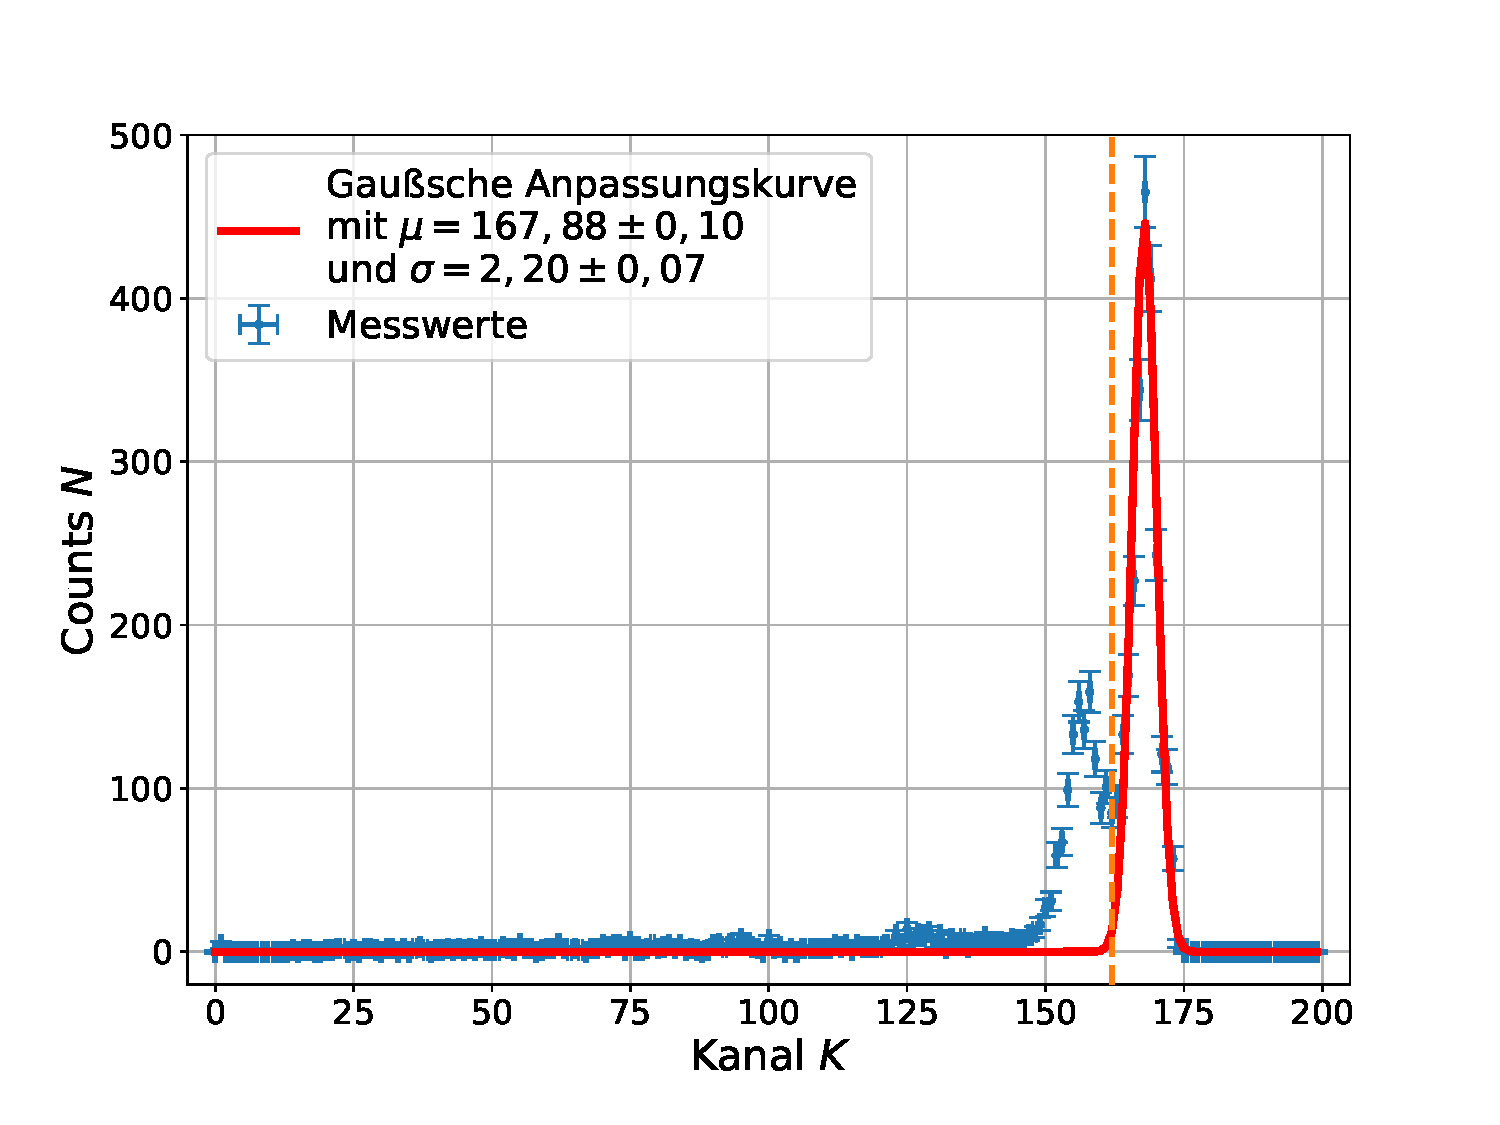
\includegraphics[width=0.7\textwidth]{src/EDetectorCalibrationChannelSpectrumEDetector}
	\caption{Die Abbildung zeigt das bei der Kalibrationsmessung des $E$-Detektors entstandene und mit diesem aufgenommene $\alpha$-Energiespektrum. Hierbei werden die Energien auf der $x$-Achse dieses Diagramms als Kanäle $K$ ausgedrückt.}
	\label{EDetectorCalibrationChannelSpectrumEDetector}
\end{figure}
Dabei stellen die sich auf der $x$-Achse dieses Diagramms befindenden Kanäle $K$ des CAMAC ADC die Energien der $\alpha$-Teilchen dar.
Die Unsicherheit jedes Kanals $K$ ist auf das Fehlerintervall $\pm 0,5$ zurückzuführen.
Weil die Unsicherheit $\sigma(N)$ der Counts $N$ auf einer Poisson-Verteilung beruht, gilt $\sigma(N)=\sqrt{N}$.
Im $\alpha$-Energiespektrum in Abbildung \ref{EDetectorCalibrationChannelSpectrumEDetector} sind zwei deutliche Peaks zu erkennen.
Der linke Peak stammt von $\alpha$-Teilchen mit einer Energie von \SI{5442,86 +- 0,12}{\kilo\electronvolt}, welche von $^{241}$Am mit einer Wahrscheinlichkeit von \SI{13,2 +- 0,1}{\percent} ausgesendet werden.
Der rechte Peak basiert auf den mit einer Wahrscheinlichkeit von \SI{84,5 +- 0,1}{\kilo\electronvolt} emittierten $\alpha$-Teilchen, welche eine Energie von $E_{0}=\SI{5485,56 +- 0,12}{\kilo\electronvolt}$ besitzen.
Da lediglich der rechte Peak für die Kalibration des $E$-Detektors relevant ist, wird eine gaußsche Anpassungskurve mit der Gestalt
\begin{align} \label{Gaussian}
f(x)=A\cdot\exp\left( -\frac{(x-\mu)^2}{2\sigma ^2}\right) + B
\end{align}
an diesen Peak gefittet.
Dabei werden nur die Messwerte berücksichtigt, welche sich im $\alpha$-Energiespektrum rechts von der orangefarbenen, gepunkteten, vertikalen Linie befinden.
Die sich ergebene gaußsche Anpassungskurve und die dazugehörigen Werte der für die Kalibration des $E$-Detektors notwendigen Fit-Parameter sind im $\alpha$-Energiespektrum in Abbildung \ref{EDetectorCalibrationChannelSpectrumEDetector} zu sehen.
Nun kann man dem Mittelwert $\mu$ die Energie $E_{0}$ zuordnen, wobei die Breite $\sigma$ der Gauß-Kurve die Detektorgrnauigkeit angibt und im Folgenden die Standartabweichung von $\mu$ bildet.
Eigentlich handelt es sich bei einem $\alpha$-Energiespektrum um ein diskretes Linienspektrum, weshalb man annehmen kann, dass die zu betrachtende \SI{5485,56 +- 0,12}{\kilo\electronvolt}-Linie im $\pm 1\sigma$-Bereich des rechten Peaks liegt.
Nimmt man zusätzlich an, dass der Kanal $K=\SI{0}{}$ der Energie $E=\SI{0}{\kilo\electronvolt}$ entspricht, so lässt sich die lineare Relation $E(K) = \SI{32,68}{\kilo\electronvolt} \cdot K$ zwischen Kanalnummer und gemessener Energie herstellen.

\subsection{Kalibration des $\Delta E$-Detektors} \label{KalidEDet}

Bei der Kalibration des $\Delta E$-Detektors wird auf ähnliche Art und Weise wie in \cref{KaliEDet} vorgegangen.
Die Abbildungen \ref{fig:kalibration_dE-_E_channel} zeigen die mit dem $E$- und dem $\Delta E$-Detektor aufgenommenen $\alpha$-Energiespektren, welche im Zuge der Kalibrationsmessung des $\Delta E$-Detektors entstanden sind.

\begin{figure}[ht]
	\centering
	\begin{subfigure}[c]{0.45\textwidth}		
		\centering	
		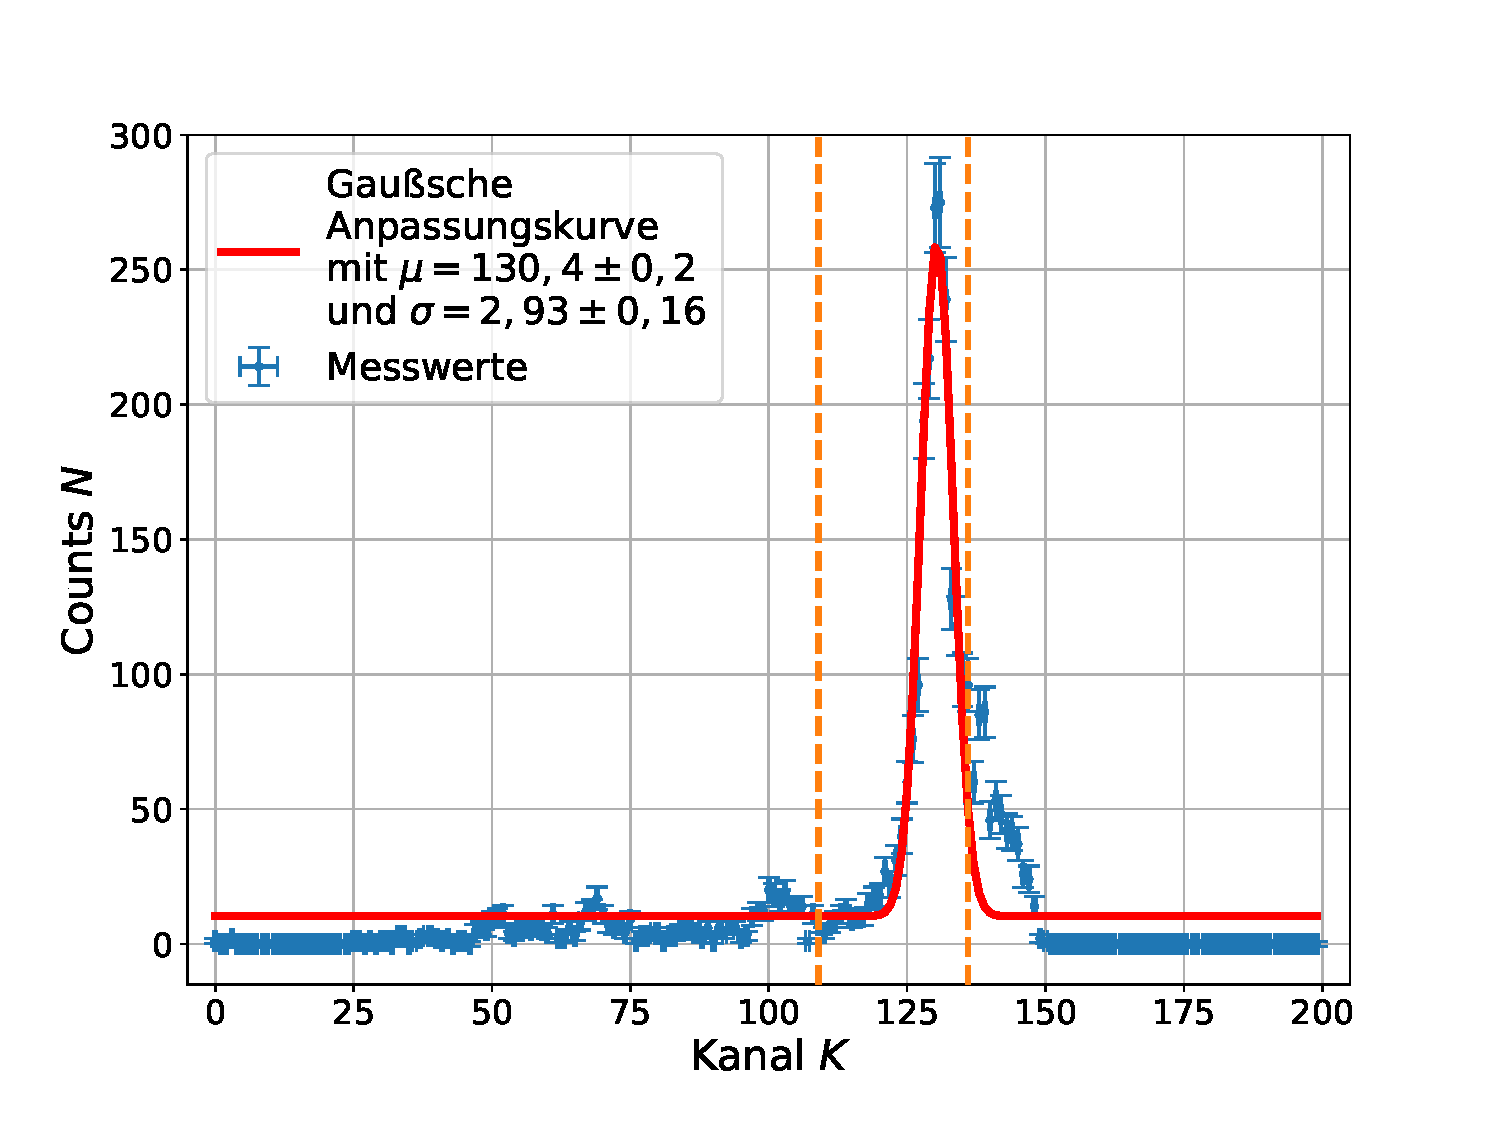
\includegraphics[width=\textwidth]{src/dEDetectorCalibrationChannelSpectrumEDetector}
		\subcaption{$E$-Detektor}
		\label{fig:kalibration_E}		
	\end{subfigure}
	\begin{subfigure}[c]{0.45\textwidth}
		\centering
		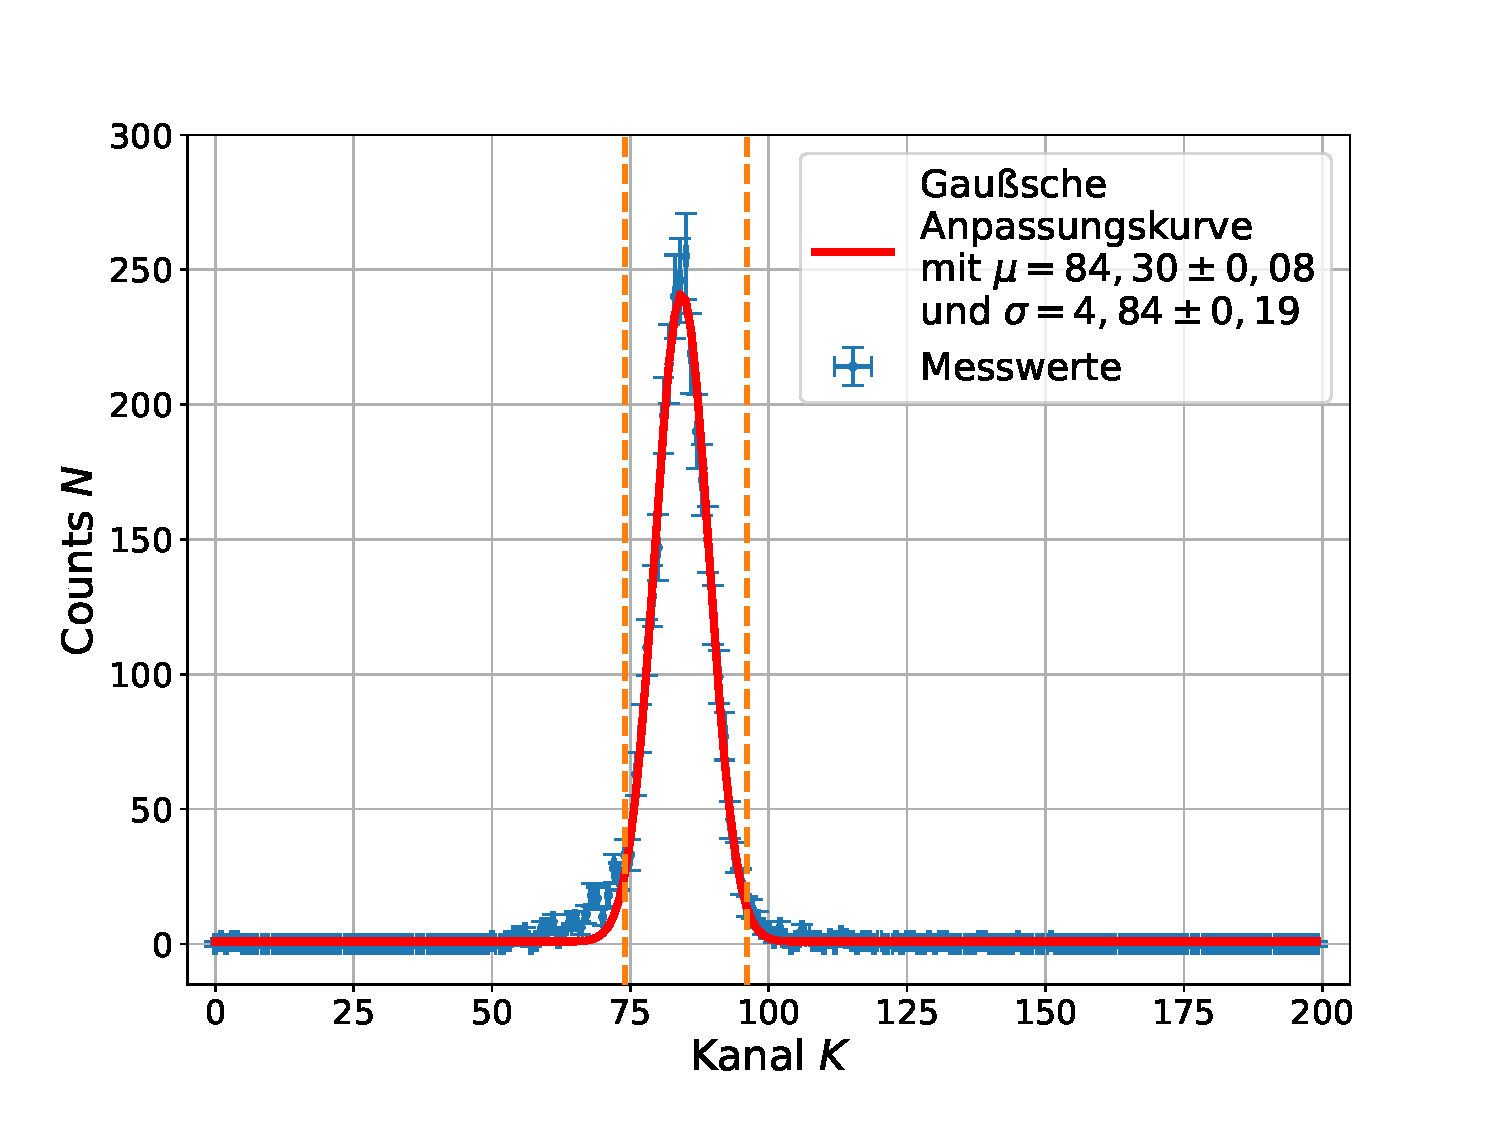
\includegraphics[width=\textwidth]{src/dEDetectorCalibrationChannelSpectrumdEDetector}
		\subcaption{$\Delta E$-Detektor}
		\label{fig:kalibration_dE}
	\end{subfigure}
	
	\caption{Die Abbildung zeigt das im Zuge der Kalibrationsmessung des $\Delta E$-Detektors aufgenommene $\alpha$-Energiespektrum. Hierbei werden die Energien auf der $x$-Achse dieses Diagramms als Kanäle $K$ ausgedrückt.
		Links das aufgenommene Spektrum des $E$-Detektors. Rechts das aufgenommene Spektrum des $\Delta E$-Detektors.}
	\label{fig:kalibration_dE-_E_channel}
\end{figure}

In beiden $\alpha$-Energiespektren lässt sich jeweils ein Peak erkennen.
An die von beiden orangefarbenen, gepunkteten, vertikalen Linien eingegrenzten Messwerte kann man nun mit Hilfe der Gleichung (\ref{Gaussian}) eine gaußsche Anpassungskurve fitten.
Die gaußschen Anpassungskurven und die dazugehörigen Werte der für die Kalibration des $\Delta E$-Detektors notwendigen Fit-Parameter sind in den Abbildungen angegeben.
Beim Passieren des $\Delta E$-Detektors erleiden die \SI{5485,56 +- 0,12}{\kilo\electronvolt}-$\alpha$-Teilchen einen Energieverlust, welcher der Position $\mu$ des Peaks im $\alpha$-Energiespektrum des $\Delta E$-Detektors entspricht.
Der Wert für diesen Energieverlust lässt sich über die Differenz zwischen den Positionen der Peaks im $E$-Detektor \cref{fig:kalibration_E} und \cref{EDetectorCalibrationChannelSpectrumEDetector} sowie unter Verwendung der Kalibrationskurve für den $E$-Detektor berechnen.
Erneut wird angenommen, dass man dem Kanal $K=\SI{0}{}$ die Energie $E=\SI{0}{\kilo\electronvolt}$ zuordnen kann, sodass sich für den $\Delta E$-Detektor die Kalibrationsgerade $\Delta E(K) = \SI{14,54}{\kilo\electronvolt} \cdot K$ ergibt.

\subsection{Dickebestimmung des $\Delta E$-Detektors} \label{sec:de_kalibration}

Im Folgenden soll die Dicke des $\Delta E$-Detektors ermittelt werden.
Dazu werden zunächst die aus dem Anhang der Versuchsanleitung\cite{wwu} entnommenen Werte für den Energieverlust von $\alpha$-Teilchen in Silizium gemäß der Vorschrift
\begin{align}
	\dv{E}{x}= \left( \dv{E}{x}\right)_\text{Elektron} + \left(\dv{E}{x}\right)_\text{Kern}
\end{align}
addiert.
Dabei ist der Energieverlust durch Kernwechselwirkung bedeutend kleiner als der durch Elektronenwechselwirkung, da es sich bei $\alpha$-Teilchen um leichte Kerne handelt, welche eine kleine Ordnungszahl besitzen.
Trägt man die im Zuge dessen erhaltenen Werte für den Energieverlust gegen die Energie $E$ des $\alpha$-Teilchens auf, ergibt sich das in Abbildung \ref{EnergyLossSpectrum} zu sehende Diagramm.
\begin{figure}[ht]
	\centering
	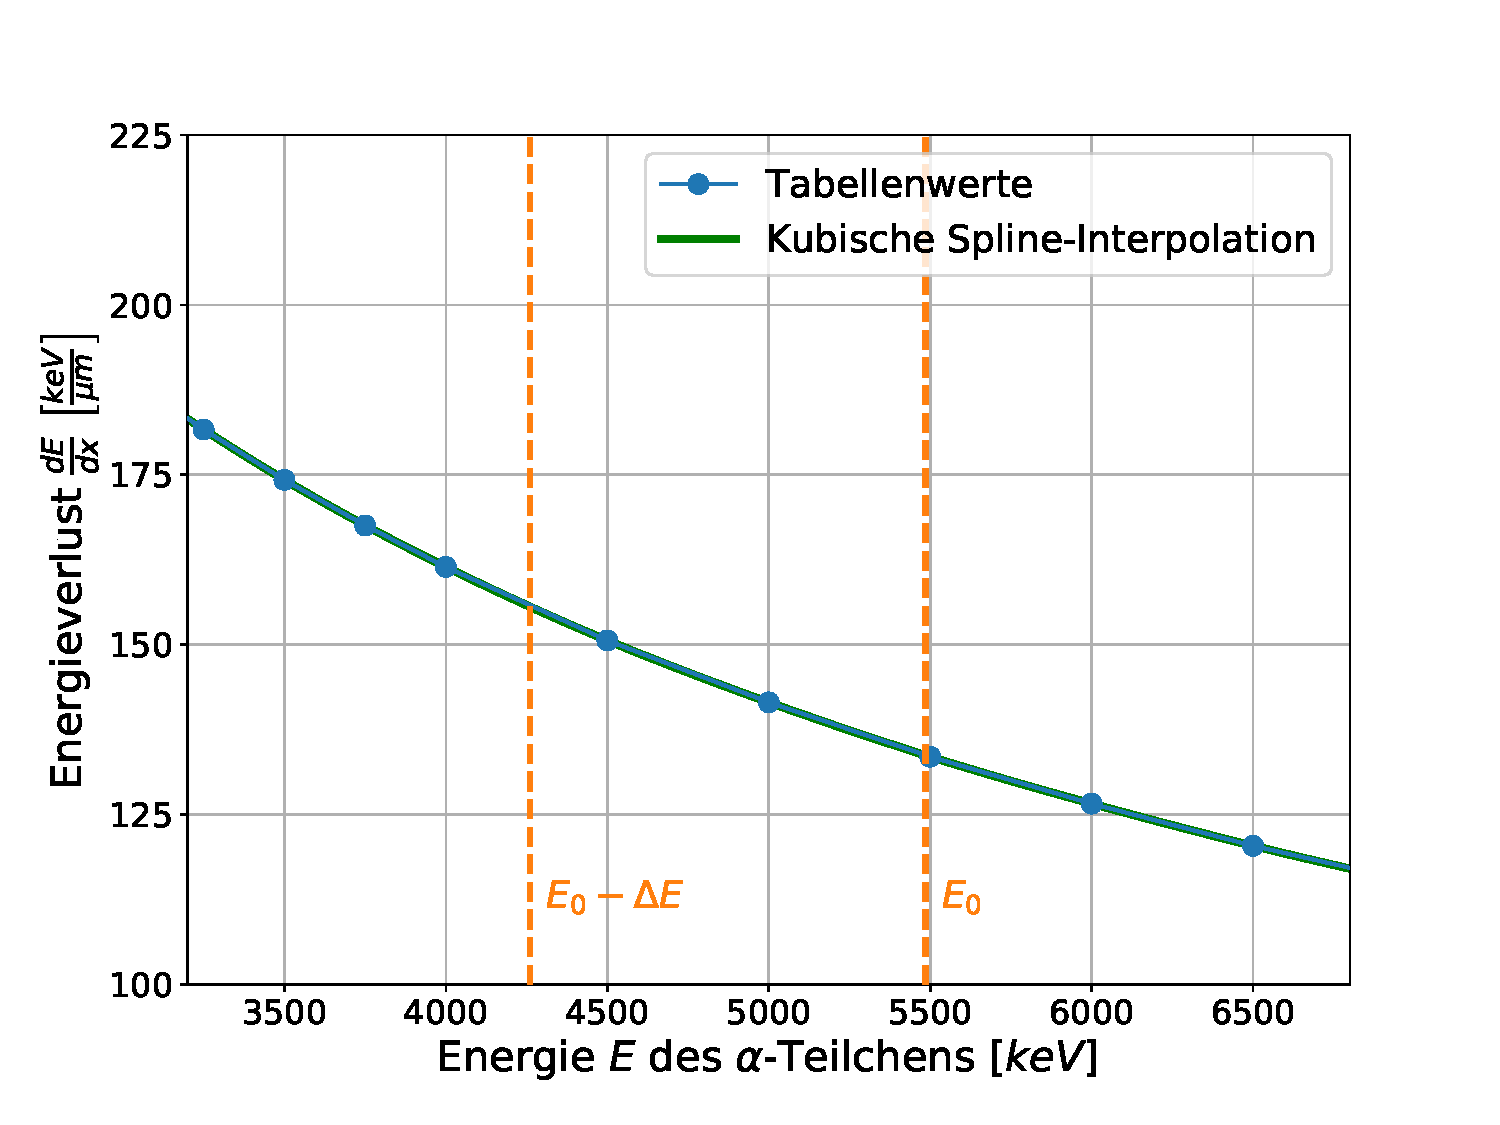
\includegraphics[width=0.7\textwidth]{src/EnergyLossSpectrum}
	\caption{Das in dieser Abbildung dargestellte Diagramm veranschaulicht den Energieverlust $\dv{E}{x}$ von $\alpha$-Teilchen in Silizium als Funktion der Energie $E$ des $\alpha$-Teilchens. Hierbei ist ein Energiebereich von \SIrange{3200}{6800}{\kilo\electronvolt} zu sehen.}
	\label{EnergyLossSpectrum}
\end{figure}
Mithilfe eines kubischen Spline-Algorithmus\footnote{Hierbei wird in python die Funktion \texttt{scipy.interpolate.interp1d} mit dem Parameter \texttt{kind="cubic"} genutzt.} wird nun eine Interpolation der Tabellenwert vorgenommen.
Die dadurch zustande kommende Kurve ist ebenfalls im Diagramm in Abbildung \ref{EnergyLossSpectrum} dargestellt.
Über numerische Integration des Ausdrucks
\begin{align}
	\Delta E = \int_{0}^{d} \dv{E}{x} (E) \dd x \approx \sum_i \dv{E}{x} (E_i) \cdot \delta x
\end{align}
lässt sich die Dicke $d$ des $\Delta E$-Detektors bestimmen.
Es wird so lange integriert, bis die Energie des Teilchens die gemessene Energie aus \cref{fig:kalibration_E} unterschritten hat.
Mit $\delta x = \SI{1e-4}{\micro\meter} = \const$ ist die zurückgelegte Strecke $d = N \cdot \delta x$, wobei $N$ die Anzahl an benötigten Integrationsschritten ist.
Man erhält für die Dicke des $\Delta E$-Detektors einen Wert von $d=\SI{8,5257}{\micro\meter}$. 

\subsection{Dickebestimmung der Mylar-Folien}
\label{sec:dicke}

Um die Dicken der Mylar-Folien zu bestimmen, werden zunächst die Restenergien der Teilchen nach Passieren der Folien bestimmt.
Dazu wird der $\Delta E$ - Detektor aus dem Strahlengang gedreht und das Energiespektrum der transmittierten Teilchen aufgenommen.
Als Referenz wird hier die Kalibrationsmessung ohne Folie verwendet.
In \cref{fig:foliendicke} sind die vier Messungen normiert nebeneinander eingezeichnet.
Alle konkreten Fitparameter der Doppelgaußkurven sind in \cref{tab:fitval1} angegeben.
Im Diagramm ist ein einzelner stark abweichender Datenpunkt bei \SI{4000}{\kilo\electronvolt} auffällig, welcher auf statistische Schwankungen zurückzuführen ist.

\begin{figure}[ht]
	\centering
	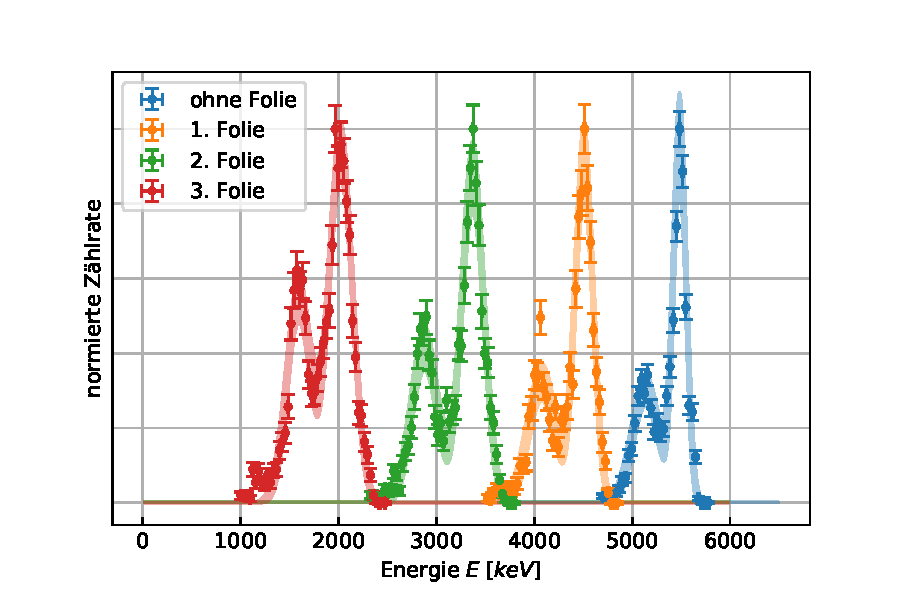
\includegraphics[width=0.7\textwidth]{dat/m3_foliendicke.pdf}
	\caption{Energiespektren nach Passieren der einzelnen Folien.
			Die Zählrate ist normiert, um die Folien besser zu vergleichen.
			Es werden nur die Datenpunkte im Bereich um den Energiepeak ungleich Null angezeigt.
			Über die Daten ist ein Doppelgauß gelegt, welcher die Parameter in \cref{tab:fitval1} annimmt und mit einer Unsicherheit $\pm 3 \sigma$ eingezeichnet ist.}
	\label{fig:foliendicke}
\end{figure}

Für die Analyse sind nur die Positionen der größeren Peaks wichtig.
Diese gehören zur \SI{5485}{\kilo\electronvolt} $\alpha$-Strahlung der Probe.
Der Detektor hat eine begrenzte Messgenauigkeit welche sich durch die Breite der Peaks widerspiegelt.
Um diese zu beachten, wird die Unsicherheit der Position $E_1$ mit der Breite $\sigma_1$ nach Formel (\ref{fig:GUM_combine}) kombiniert.

Nun wird eine numerische Integration durch die Folien durchgeführt.
Dazu wird zunächst der Energieverlust $\dv{E}{x}$ von $\alpha$-Teilchen in Mylar aus der Anleitung interpoliert.
Für ein eintreffendes Teilchen mit \SI{5485}{\kilo\electronvolt} kann nun schrittweise der Energieverlust $\dd E_i = \dv{E}{x} \left(E_i\right) \cdot \delta x$ berechnet werden.
Mit $\delta x = \SI{1e-4}{\micro\meter} = \const$ ist die zurückgelegte Strecke $\bar{x} = N \cdot \delta x$, wobei $N$ die Anzahl an benötigten Integrationsschritten ist.
Um die Standardabweichung für die Dicken zu bestimmen, wird die Integration ebenfalls für $E_1^\pm = \bar{E_1} \pm \sigma(E_1)$ durchgeführt.
Nun wird mit den zu $E_1^\pm$ gehörenden Dicken $x^\pm$ die gemittelte Differenz $\sigma(x) = \frac{x^+ - x^-}{2}$ gebildet.
Die ermittelten Energien und Dicken der Folien sind in \cref{tab:dicken} zusammengefasst.

\begin{table}[ht]
	\centering
	\caption{Energien der Teilchen nach Passieren der Folien und die errechneten Dicken dieser.} 
	\label{tab:dicken}
	\begin{tabular}{c|ccc}
		\toprule
		         &          Energie $E_1$          &           Dicke $x$           &  \\ \midrule
		1. Folie & \input{dat/folie_energie_1.txt} & \input{dat/folie_dicke_1.txt} &  \\
		2. Folie & \input{dat/folie_energie_2.txt} & \input{dat/folie_dicke_2.txt} &  \\
		3. Folie & \input{dat/folie_energie_3.txt} & \input{dat/folie_dicke_3.txt} &  \\ \bottomrule
	\end{tabular}
\end{table}

Aus den bestimmten Dicken könnte man schließen, dass die Folien Vielfache von \SI{8}{\micro\meter} dick sind und im Falle der 1. und 2. Folie um ca. \SI{13}{\degree} gedreht sind oder keine gleichmäßige Dicke aufweisen.
Diese Angaben sind allerdings nicht zu überprüfen und sind als Spekulationen zu betrachten.
Um die Unsicherheit zu erhöhen, muss die Detektorgenauigkeit erhöht werden.
Dies kann zum Beispiel über eine Faltung mit der Detektorverteilung einer wohlbekannten Kalibrationsmessung erzielt werden.

\subsection{Bestimmung des Energieverlusts}

Um die Teilchenidentifikation durchzuführen, werden alle aufgenommenen Messungen aufaddiert und in ein Diagramm geschrieben.
Dabei ist die Energie des Teilchens die Summe von gemessener Restenergie im $E$-Detektor und deponierter Energie im $\Delta E$-Detektor.
Die Messdaten, sowie theoretisch errechnete Kurven für Protonen, Deuteronen, Tritonen, Helium-3-Kerne, $\alpha$-Teilchen und Lithium-Kerne sind in \cref{fig:energieverlust} dargestellt.

\begin{figure}[ht]
	\centering
	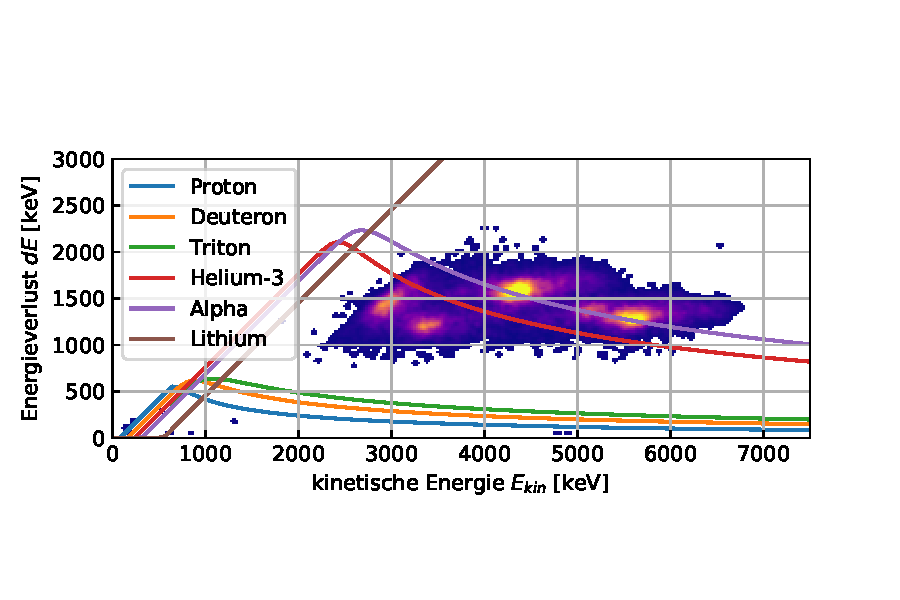
\includegraphics[width=0.7\textwidth]{dat/energieverlust.pdf}
	\caption{Energieverlust $\Delta E$ von Teilchen der Energie $E$. Zusätzlich sind die theoretisch erwarteten Kurven für sechs Teilchensorten eingezeichnet.}
	\label{fig:energieverlust}
\end{figure}

Man kann erkennen, dass die theoretische Kurve für $\alpha$-Teilchen durch die beiden hellsten Punkte sowie durch einen weiteren Häufungspunkt bei $E=\SI{5100}{\kilo\electronvolt}$ verläuft.
Allerdings liegen die beiden Punkte bei $E = \SI{3000}{\kilo\electronvolt}$ und $E=\SI{3400}{\kilo\electronvolt}$ nicht auf der theoretischen Kurve.
Auch Helium-3 könnte im weitergehenden Zusammenhang ein Kandidat der verwendeten Teilchenart sein, da dessen Kurve ebenfalls in dem Gebiet der Messung liegt.

Um die theoretischen Kurven zu berechnen, ist die Bethe Bloch Formel nach \cref{eq:bethebloch} für Silikon implementiert worden.
Nun kann wie in \cref{sec:dicke} eine schrittweise Integration durch den Detektor durchgeführt werden.
Die Abbruchbedingung ist diesmal die Dicke des Detektors $d = \SI{8.5257}{\micro\meter}$, welche aus \cref{sec:de_kalibration} bekannt ist.

Um zu entscheiden, ob nun $\alpha$-Teilchen oder Helium-3 Kerne vorliegen, wird der gesamte Datensatz auf $\Delta \cdot \beta^2$ projiziert und als Histogramm dargestellt.
Dabei wird in $\beta$ die Masse $M$ des Teilchens benötigt und man muss für jedes zu überprüfende Teilchen eine eigene Verteilung erstellen.
Auch hier wird wieder ein theoretischer Kurvenverlauf benötigt.
Der Mittelwert der Kurve kann mit $E = \SI{5485}{\kilo\electronvolt}$ und dem Energieverlust $\Delta E$, welcher durch der oben genannten Integration bekannt ist, bestimmt werden.
Die Breite der Gaußkurve wird hier als konstant angesehen und entsprechend der Detektorgenauigkeit gewählt.
In \cref{fig:debeta} sind die beiden Verteilungen für $\alpha$-Teilchen und Helium-3 Kerne eingezeichnet.
Andere Teilchenarten sind in \cref{fig:debeta_full} gegeben.

\begin{figure}[ht]
	\centering
	\begin{subfigure}[c]{0.45\textwidth}
		\centering
		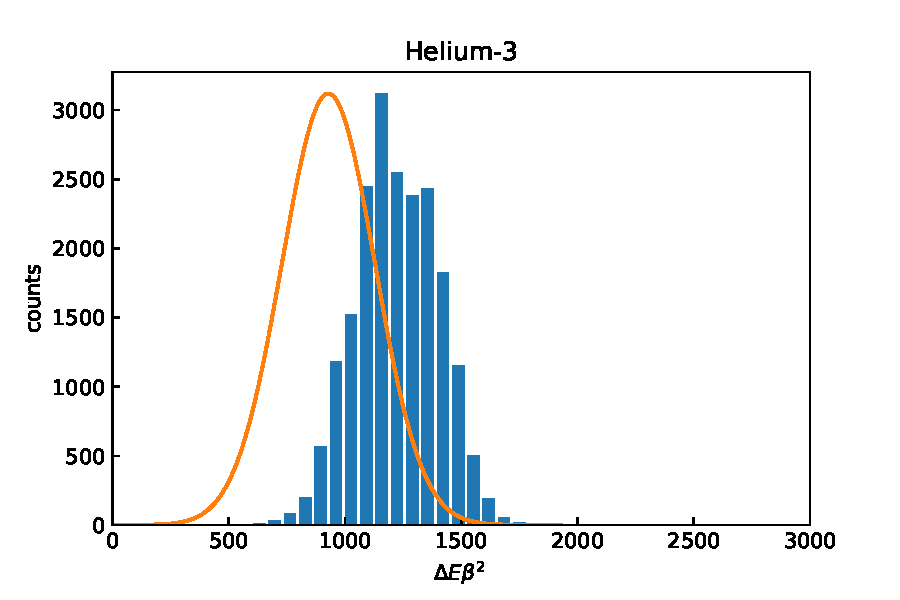
\includegraphics[width=\textwidth]{dat/debeta_Helium-3.pdf}
	\end{subfigure}
	\begin{subfigure}[c]{0.45\textwidth}
		\centering
		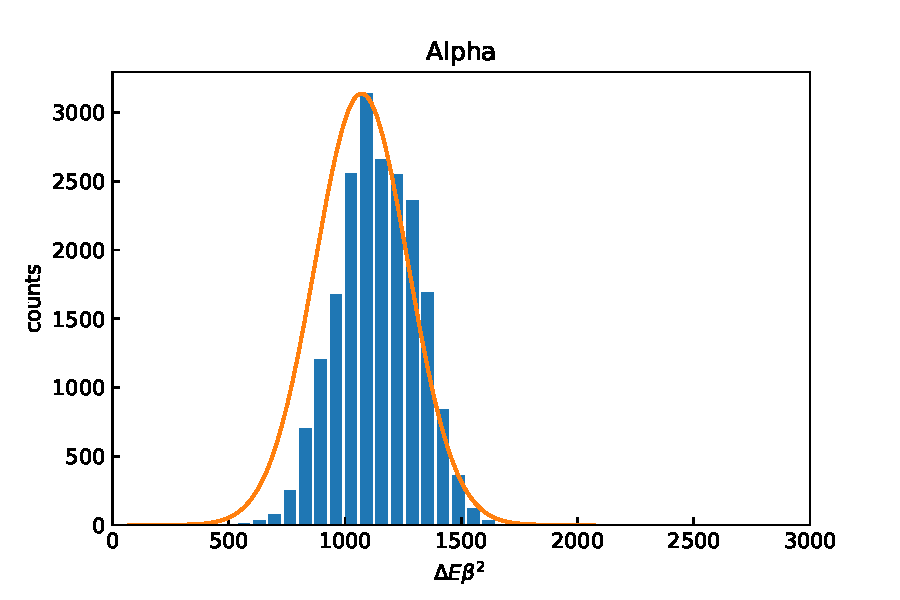
\includegraphics[width=\textwidth]{dat/debeta_Alpha.pdf}
	\end{subfigure}
	\caption{$\Delta E \beta^2$ Verteilungen für $\alpha$-Teilchen und Helium-3 Kerne. Eingezeichnet sind die gemessenen Werte, sowie die theoretisch zu erwartenden Verteilungen.}
	\label{fig:debeta}
\end{figure}

Man kann erkennen, dass die theoretische Verteilung der $\alpha$-Teilchen am besten auf den gemessenen Daten liegt.
Abschließend lässt sich zusammenfassen, dass es sich bei den abgestrahlten Teilchen des Americium-241 tatsächlich um $\alpha$-Teilchen handelt.
